% Este archivo es parte de la memoria del proyecto fin de carrera
% de Manuel López Urbina. Protegida bajo la licencia GFDL.
% Para más información, la licencia completa viene incluida en el
% fichero fdl-1.3.tex

% Copyright (C) 2018 Manuel López Urbina

\newpage


\chapter{Organización temporal}
\label{chap:planificación}

La planificación general del proyecto siguiendo un modelo SCRUM, empleando para ello el panel de tareas Trello; un gestor de proyectos que permite aplicar una metodología de desarrollo ágil.\\

\begin{figure}[H]
\hspace*{-.2in}{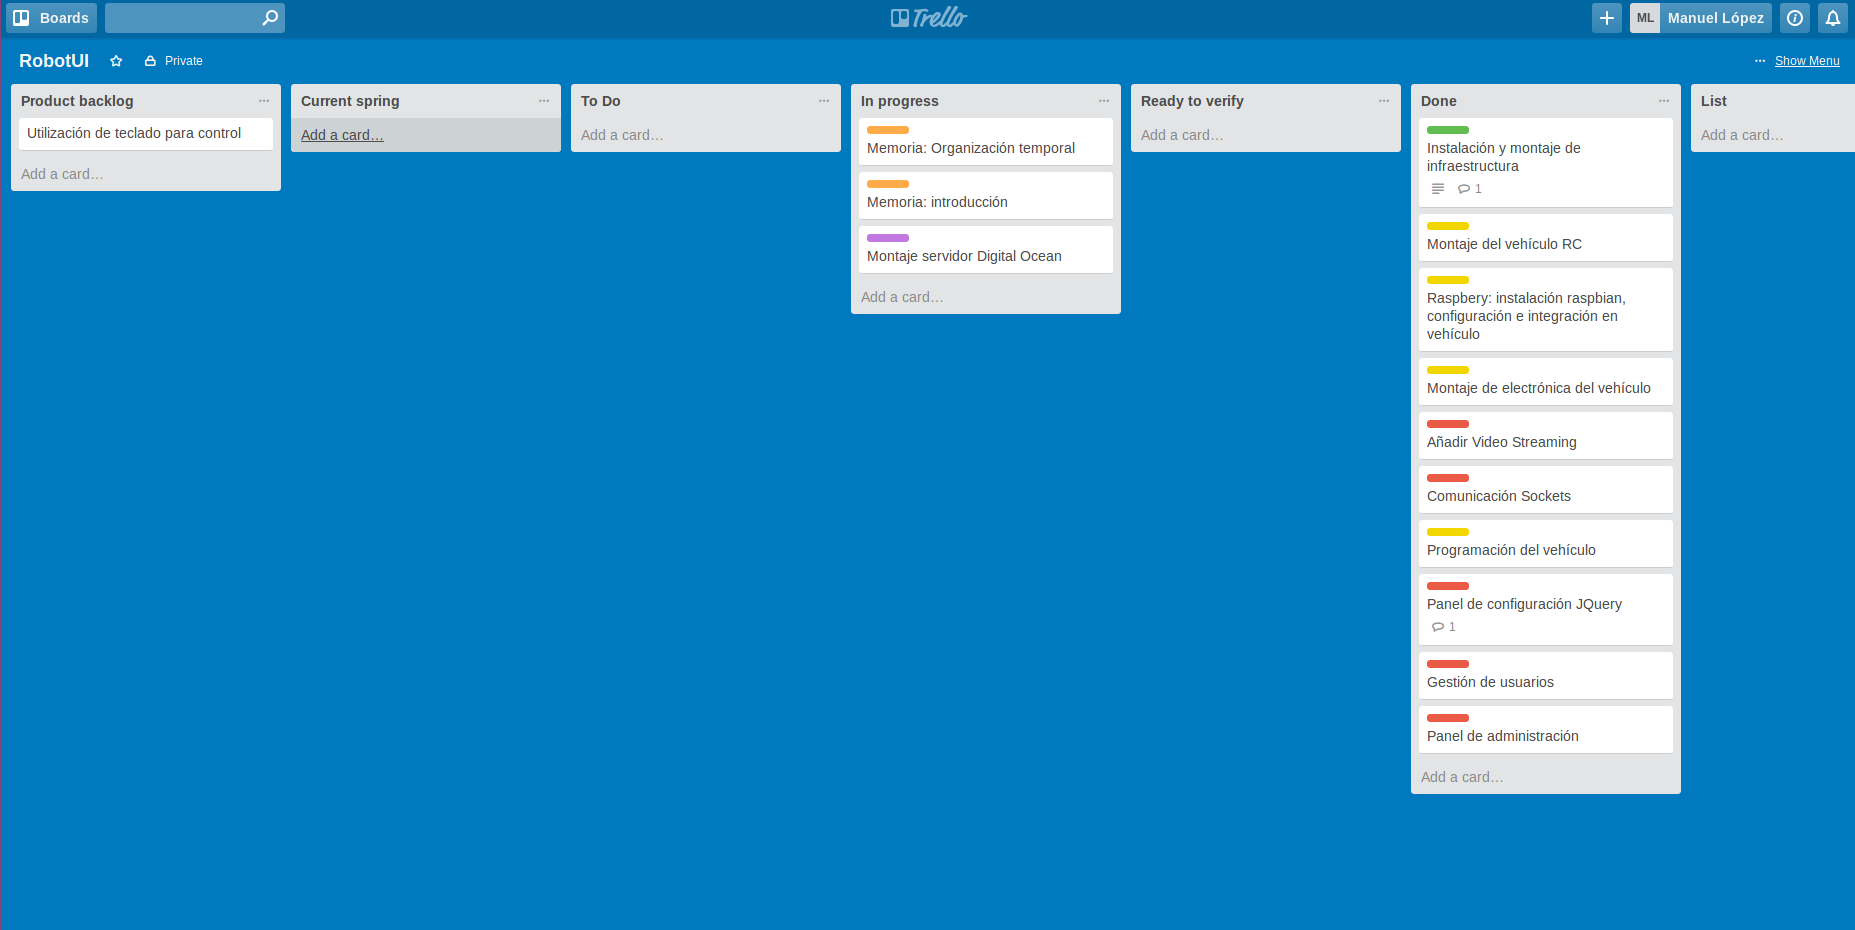
\includegraphics[scale=0.25]{imagenes/panel-trello.png}}
\caption{Panel de actividades - Trello}
\end{figure}

Cabe destacar que para el desarrollo de SensorRS ha sido necesario emplear varias herramientas, utilidades y bibliotecas. Algunas de ellas ya habían sido utilizadas en ciertas
ocasiones, bien sea en el ámbito estudiantil o profesional. Sin embargo, otras han requerido un periodo de formación previo, en el que se han adquirido los conocimientos necesarios
para poder desarrollar el presente proyecto.\\

La mayor parte del proceso de investigación fue dedicado al estudio de las diferentes tecnologías referentes a la programación de microcontroladores e interconexión de elementos
electrónicos. Todo ello ha implicado un esfuerzo bastante considerable en el uso, aprendizaje e investigación de las diferentes tecnologías existentes y comprobar su potencial.\\

Una vez determinadas las diferentes herramientas a utilizar se comenzó con la implementación comenzando por la programación de ejemplos básicos en Arduino.\\

La figura \ref{gantt:tareas01} muestra una visión de las diferentes tareas desarrolladas para la elaboración del proyecto junto con la descomposición de cada una de ellas:\\

\begin{figure}
  \begin{center}
    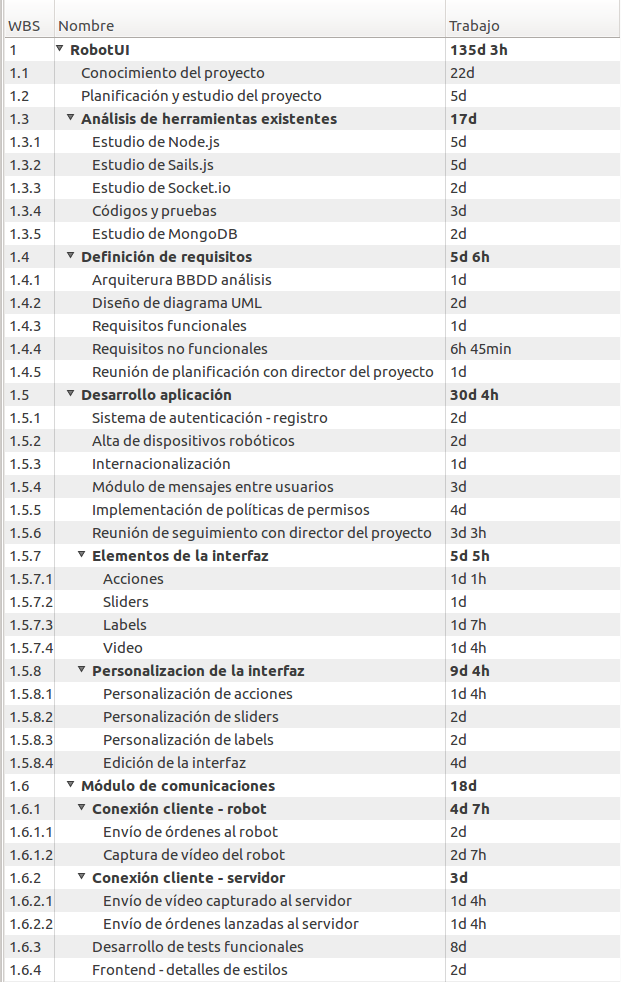
\includegraphics[scale=0.6]{imagenes/planificacion/descomposicion_tareas01.png}
  \end{center}
  \caption{Descomposición de las tareas implicadas en la construcción del vehículo robótico SensorRS (Primera Parte).}
  \label{gantt:tareas01}
\end{figure}

Los puntos más importantes del proyecto se han dividido en hitos, así como entregas que se definieron en cada reunión que se realizaba con el director del proyecto. 
También se ha definido una planificación temporal del desarrollo del proyecto mediante un diagrama de Gantt con la duración de las tareas recogidas en el panel de actividades de Trello.\\
\newpage

\section{Planificación temporal de tareas}
\chaptermark{Planificación}

A continuación se definirán los diferentes hitos que componen el diagrama de Gantt divididos en las diferentes subtareas principales de cada uno de ellos:\\

\subsection{Hito 1: Planificación y análisis }
\label{subsec:hito1}

En esta primera etapa de desarrollo del proyecto final de carrera se realizaron los estudios previos necesarios para abordar cualquier proyecto de cierta envergadura.\\

Este hito se descompone en las siguientes tareas principales:

\begin{enumerate}
 \item Planificación y estudio del proyecto. En esta fase se centró en la elaboración de un documento, a modo borrador, con la idea a desarrollar, objetivos del proyecto y su alcance.
 \item Análisis de herramientas existentes, de las tecnologías a implementar, la arquitectura del sistema, las tecnologías de BD, visualización, para la selección de las herramientas más adecuadas 
 para afrontar el desarrollo con garantías y no sea necesaria una ``vuelta atrás'' por necesidad imperiosa de cambio de tecnología. En definitiva se buscaba una herramienta libre, con un respaldo de una comunidad importante
 y que resuelva la problemática o necesidad de trabajar con sensores y transmisión de datos.
\end{enumerate}

\subsection{Hito 2: Definición de requisitos }
\label{subsec:hito2}

Este segundo hito queda dividido en las siguientes etapas:

\begin{enumerate}
 \item Elaboración de un documento formal con la propuesta de proyecto definiendo sus objetivos y alcance, para la aprobación por parte del director del proyecto.
 \item Se definen las las funcionalidades que debe cumplir el sistema, elementos electrónicos y software a utilizar, definición de requisitos funcionales y no funcionales. 
\end{enumerate}

\subsection{Hito 3: Montaje del vehículo}
\label{subsec:hito2}

En este segundo hito, uno de los de mayor magnitud, se comienza con el montaje e interconexión de los elementos hardware del vehículo, el cual queda dividido en las siguientes subtareas:\\

\begin{enumerate}
 \item Instalación del sistema operativo y software necesario en la placa Raspberry Pi.
 \item Conexión por puerto serie de la placa Arduino y Raspberry pi.
 \item Interconexión de sensores.
 \item Montaje de los elementos sobre el chasis del vehículo.
 \item Alimentación de todo el conjunto.
\end{enumerate}

Se realiza la construcción y montaje e instalación software del vehículo robótico y comprobación de las diferentes conexiones.

\subsection{Hito 4: Programación del vehículo SensorRS }
\label{subsec:hito3}

Este tercer hito comprende toda la programación lógica del vehículo dividiéndose principalmente en dos partes:

\begin{enumerate}
 \item Programación de la placa Raspberry Pi, código en Node.js para la comunicación con el servidor de control, captura de valores de la palaca Arduino y transmisión de datos.
 \item Programación de la placa Arduino.
\end{enumerate}

\subsection{Hito 5: Mejoras en la aplicación de control RobotUI }
\label{subsec:hito6}

Debido a nuevas necesidades del proyecto y diversos aspectos mejorables de la aplicación uno de los hitos del presente proyecto ha sido dedicado a la realización de estas tareas entre las que destacan:\\

\begin{enumerate}
 \item Incorporación de la posibilidad de de utilización de un Gamepad para el control de los diferentes dispositivos robóticos.
 \item Renovación de la interfaz incluyendo la última versión del popular framework Bootstrap para Html, Css y JavaScript.
 \item Mejoras en el apartado de comunicaciones estableciendo un canal específico para la transmisión de vídeo y otro para el de comando y valores de los sensores.
\end{enumerate}


\subsection{Hito 6: Documentación }
\label{subsec:hito6}

Se finaliza la memoria para la revisión por parte del director del proyecto y su posterior impresión. Se prepara la presentación para la defensa ante tribunal.

\section{Diagrama de Gantt}

A continuación se muestra el diagrama de Gantt donde quedan reflejados los diferentes hitos descritos en el punto anterior.

\begin{figure}
  \hspace*{.8in}{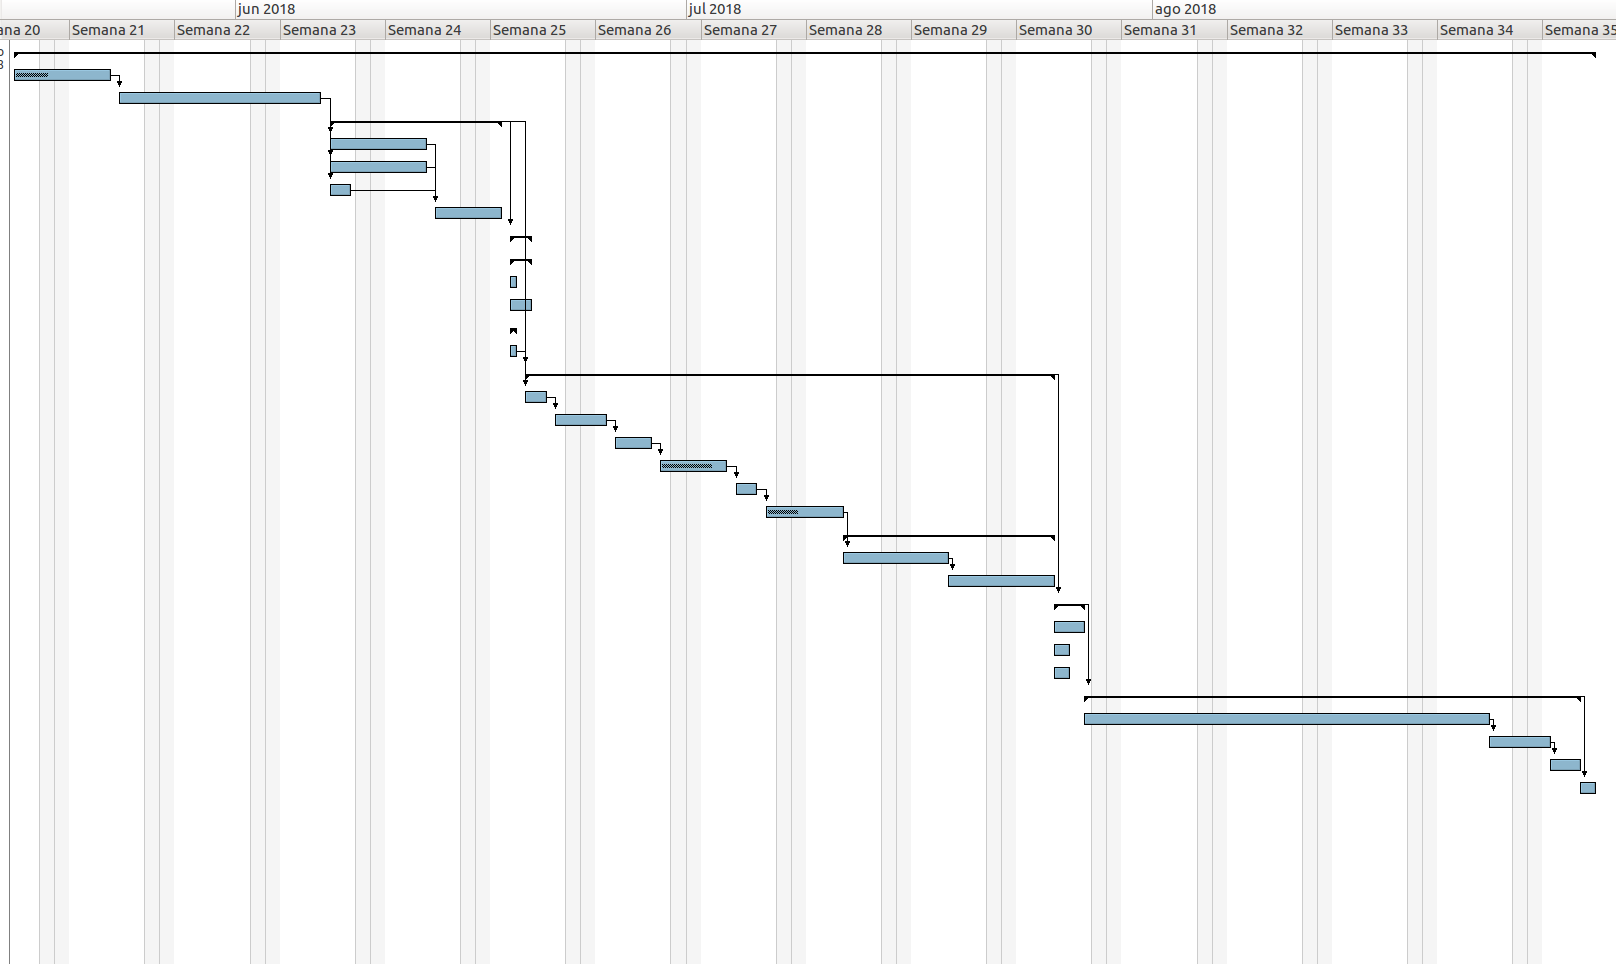
\includegraphics[scale=0.38,angle=270]{imagenes/planificacion/gantt_01.png}}
  \caption{Diagrama de Gantt. Desarrollo del proyecto.}
\end{figure}
